
\documentclass[10 pt,usenames,dvipsnames, oneside]{article}
\usepackage{../../modelo-fracoes}
\graphicspath{{../../../Figuras/licao04/}}


\begin{document}

\begin{center}
  \begin{minipage}[l]{3cm}

\includegraphics[width=2cm]{../../../Figuras/logo}       
\end{minipage}\hfill
\begin{minipage}[r]{.8\textwidth}
 {\Large \scshape Atividade: O bolo da mãe da Rita}  
\end{minipage}
\end{center}
\vspace{.2cm}

\ifdefined\prof
%Caixa do Para o Professor
\begin{goals}
%Objetivos específicos
\begin{enumerate}
\item       Comparar frações, em que os denominadores são múltiplos, a
partir de modelos contínuos.
\end{enumerate}

\tcblower

%Orientações e sugestões
\begin{itemize}
\item       Recomenda-se que, nesta atividade, os alunos trabalhem
individualmente ou em duplas. No entanto, é fundamental que os alunos sejam
estimulados a explicar o raciocínio realizado.
\item       Para amparar a reflexão dos alunos, recomenda-se que sejam
feitas cópias das             folhas para reprodução disponíveis no final do
livro.
\item       Não se recomenda que a nomenclatura       ``frações
equivalentes''       seja introduzida em sala de aula. Por exemplo, pode-se
falar apenas que as frações $\frac{1}{2}$ e $\frac{2}{4}$ representam a mesma quantidade, e por isso
têm a mesma representação na reta numérica.
\item       Esta atividade pode desencadear uma discussão com os alunos que
os leve a perceberem que se multiplicamos (dividimos) numerador e denominador de
uma fração pelo mesmo número então é gerada uma fração equivalente à fração
original.
\end{itemize}
\end{goals}

\bigskip
\begin{center}
{\large \scshape Atividade}
\end{center}
\fi

Rita convidou seus colegas de escola para virem à sua casa conhecer seu novo cãozinho. Sua mãe preparou um bolo para o lanche da tarde das crianças. Às 16h chegaram dois de seus colegas, João e Mário. Mário logo imaginou o bolo repartido em 3 pedaços e pensou que ele poderia então comer um terço do mesmo

\begin{center}
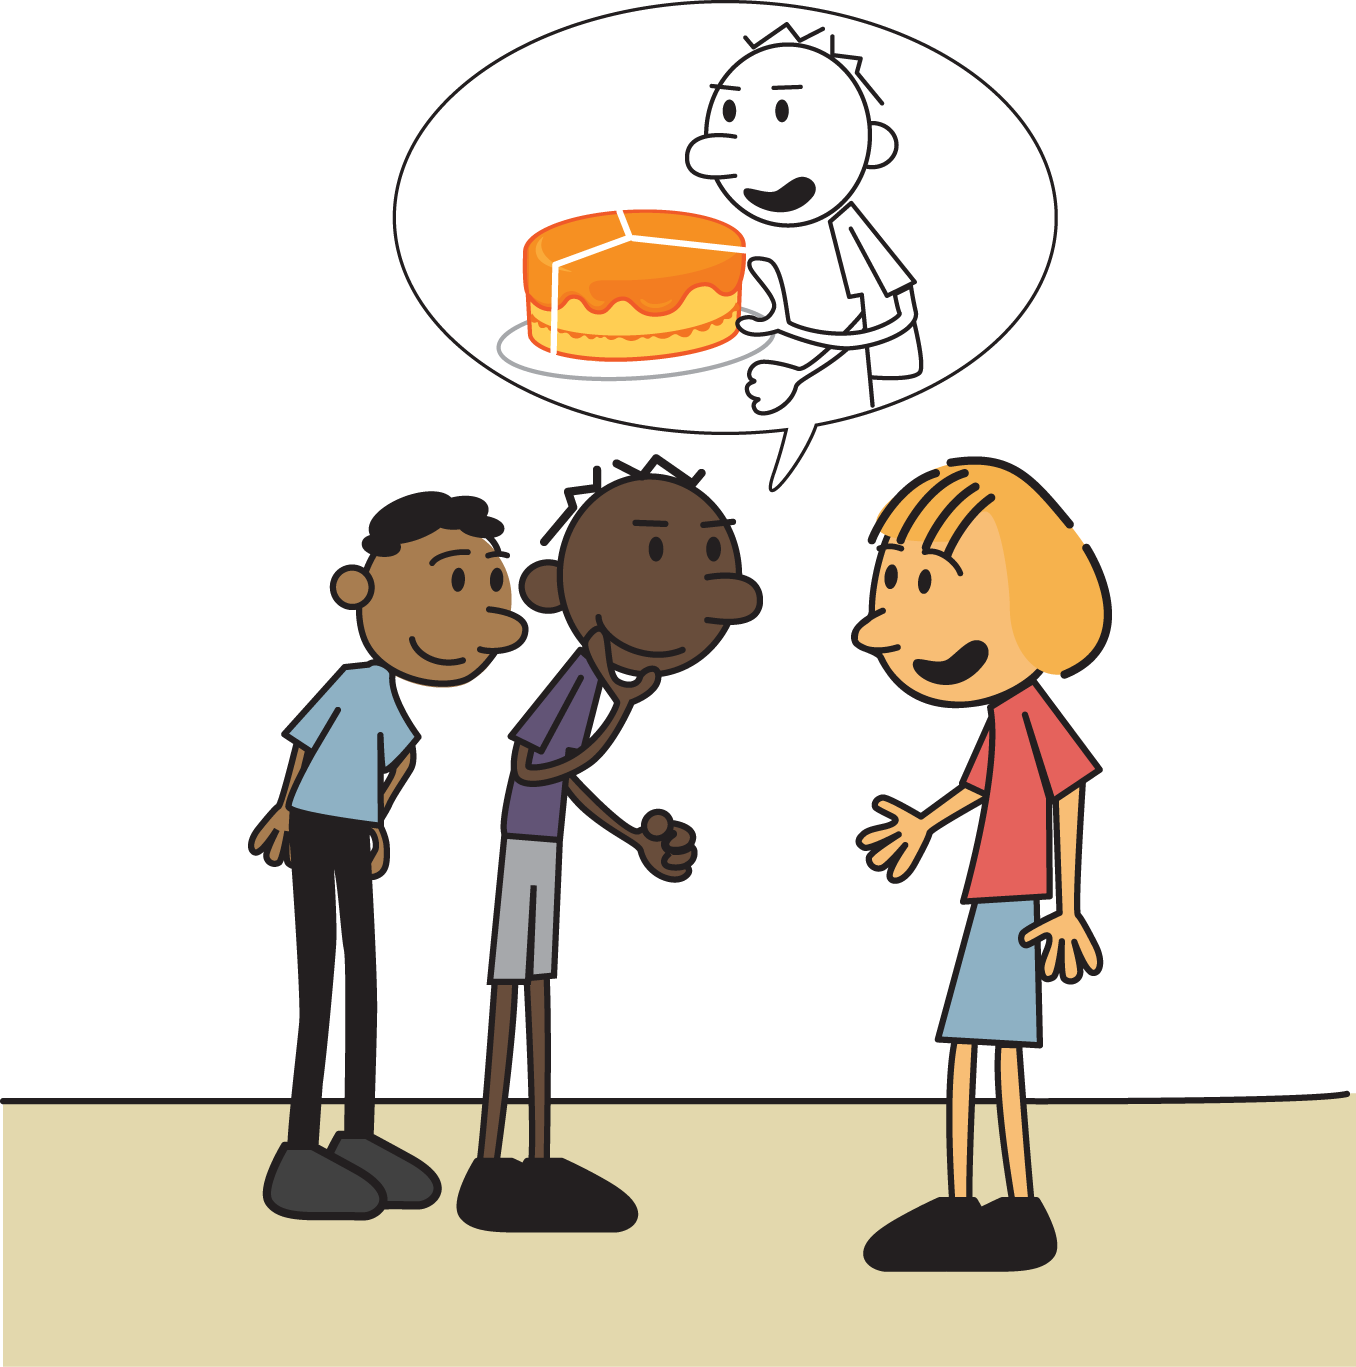
\includegraphics[width=.5\textwidth, keepaspectratio]{ativ4_fig01.png}
\end{center}

A mãe de Rita começou a cortar o bolo, partindo-o, como Mário havia imaginado, em 3 partes. No entanto, antes que começassem a comer, chegaram mais 4 colegas da escola. Então a mãe de Rita dividiu cada um dos 3 pedaços iniciais em 4 partes de igual tamanho.

\begin{center}
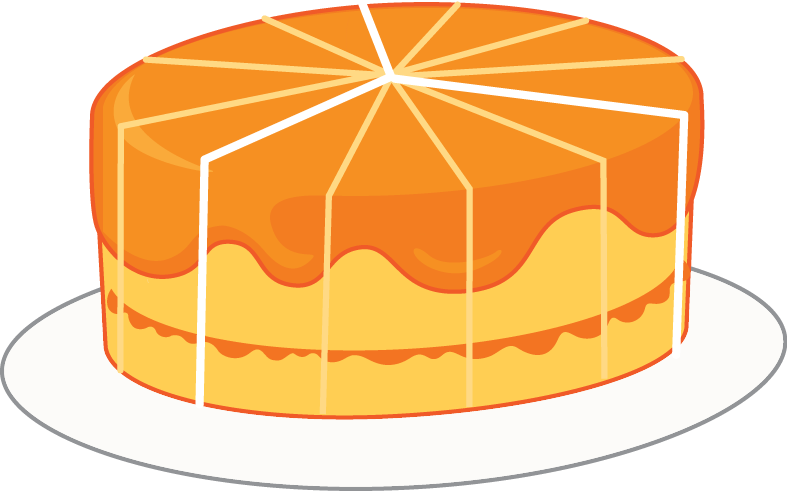
\includegraphics[width=.25\textwidth, keepaspectratio]{ativ4_fig02.png}
\end{center}



Na hora do lanche, João comeu 2 pedaços do bolo e Mário comeu 4.
\begin{itemize} %s
  \item     Que fração do bolo Mário comeu?
  \item     Que fração do bolo João comeu?
\end{itemize} %s

Se os amigos atrasados não tivessem aparecido antes do lanche, a mãe de Rita não teria subdivido as 3 fatias iniciais. Assim, se fossem apenas Rita, Mário e João, cada um teria comido $\frac{1}{3}$ do bolo.
\begin{itemize} %s
  \item     Nesse caso, Mário teria comido menos bolo, mais bolo ou a mesma quantidade de bolo que comeu?
  \item     E João, teria comido menos bolo, mais bolo ou a mesma quantidade de bolo que comeu?
\end{itemize} %s

\ifdefined\prof
\begin{solucao}

Na hora do lanche, João comeu   $\frac{2}{12}$   e Mário   $\frac{4}{12}$   do
bolo. Se os amigos atrasados não tivessem aparecido antes do lanche, João e
Mário teriam comido, cada um,   $\frac{1}{3}$   do bolo. Como   $\frac{1}{3}$
do bolo corresponde a   $4$   fatias do bolo cortado em   $12$   partes iguais,
vê-se que João teria comido mais bolo e Mário teria comido a mesma quantidade de
bolo se seus amigos não tivessem aparecido antes do lanche.

\end{solucao}
\fi

\end{document}